\section{Existing Limits}
\label{sec:HBSM_app:existinglimits}
We would like to place a limit on BR$(H\rightarrow aa\rightarrow \gamma\gamma jj) = 2\text{BR}(H\rightarrow aa)\times\text{BR}(a\rightarrow\gamma\gamma)\text{BR}(a\rightarrow jj)$,
given limits on BR$(H\rightarrow aa\rightarrow 2\gamma2\gamma)$ and BR$(H\rightarrow aa)$.

\noindent For brevity, let $B\equiv \text{BR}(H\rightarrow aa)$, $x\equiv \text{BR}(a\rightarrow\gamma\gamma)$, and $y\equiv \text{BR}(a\rightarrow jj)$.

\noindent With these conventions, we have that $B<0.34$ from~\cite{Khachatryan:2016vau}; we also have that $Bx^2<0.001$ from~\cite{Aad:2015bua}; and we would like to use this information to place a limit on $2Bxy$. 

\noindent We note first that $y\le 1-x$, with the inequality satisfied when the $a$ particle decays exclusively into photons and jets.

\noindent The following facts will be useful, which are true for any value of $x$.

\noindent First, for any $s\le\frac{1}{2}$, if $x<s$ then $x(1-x)<s(1-s)$.

\noindent Second, $x(1-x)\le \frac{1}{4}$.

\noindent We do not know the true value of $B$,
so we consider two cases which cover all possibilities: $B<0.004$, and $0.004\le B<0.34$.

\noindent If $B<0.004$, then:
\begin{align*}
2Bxy &\le 2Bx(1-x) \\
&<2\times0.004\times\frac{1}{4} \\
&=0.002
\end{align*}

\noindent If $0.004\le B<0.34$, then: 
\begin{align*}
Bx^2 &< 0.001\\
\rightarrow x&<\sqrt{\frac{0.001}{B}}\\
&\le \frac{1}{2}\\
\rightarrow x(1-x)&<\sqrt{\frac{0.001}{B}}\times\left(1-\sqrt{\frac{0.001}{B}}\right)
\end{align*}
\noindent Then we have: 
\begin{align*}
2Bxy &\le 2Bx(1-x) \\
&<2\times B\times\sqrt{\frac{0.001}{B}}\times\left(1-\sqrt{\frac{0.001}{B}}\right) \\
&=2(\sqrt{0.001B}-0.001)\\
&<2(\sqrt{0.001\times0.34}-0.001)\\
&\approx 0.035
\end{align*}

\noindent Thus no matter what $B$ is, we have $2Bxy<0.035$.

\section{Jet Kinematics}
\label{sec:HBSM_app:kinematics}
The distributions of $m_{jj}$, $|m_{jj}-m_{\gamma\gamma}|$, and $|m_{\gamma\gamma jj}$ are shown for $m_a=20$ \GeV{} (Figure~\ref{fig:HBSM:signal_kinematics_m20});
$m_a=30$ \GeV{} (Figure~\ref{fig:HBSM:signal_kinematics_m30});
$m_a=40$ \GeV{} (Figure~\ref{fig:HBSM:signal_kinematics_m40});
$m_a=50$ \GeV{} (Figure~\ref{fig:HBSM:signal_kinematics_m50});
and $m_a=60$ \GeV{} (Figure~\ref{fig:HBSM:signal_kinematics_m60}).

\begin{figure}[t]
  \centering 
  \subfloat[]{\includegraphics[width=0.45\textwidth]{figures/{mjj_shape_m20}.pdf}}
  \subfloat[]{\includegraphics[width=0.45\textwidth]{figures/{amassdiff_shape_m20}.pdf}}\\
  \subfloat[]{\includegraphics[width=0.45\textwidth]{figures/{hmasses_shape_m20}.pdf}}
  \subfloat[]{\includegraphics[width=0.45\textwidth]{figures/{hmasses_amassdiff_shape_m20}.pdf}}\\
  \caption{
    Distributions of kinematic observables before the requirements on \smash{$m_{jj}^\text{VBF}$}, leading VBF jet \pt{}, \smash{$m_{\gamma\gamma jj}$}
    and $|m_{jj}-m_{\gamma\gamma}|$ for:
    (a) $m_{jj}$;
    (b) $|m_{jj}-m_{\gamma\gamma}|$;
    (c) $m_{\gamma\gamma jj}$;
    and (d) $m_{\gamma\gamma jj}$ (with the additional requirement $|m_{jj}-m_{\gamma\gamma}|< x_\text{R}$ that defines the signal-enriched region).
    The quantities are shown separately for simulated signal events (with $m_a=20$ \GeV{}) produced in the VBF mode 
    and compared with those produced in the ggF mode and the observed data.
    }
  \label{fig:HBSM:signal_kinematics_m20}
\end{figure}

\begin{figure}[t]
  \centering 
  \subfloat[]{\includegraphics[width=0.45\textwidth]{figures/{mjj_shape_m30}.pdf}}
  \subfloat[]{\includegraphics[width=0.45\textwidth]{figures/{amassdiff_shape_m30}.pdf}}\\
  \subfloat[]{\includegraphics[width=0.45\textwidth]{figures/{hmasses_shape_m30}.pdf}}
  \subfloat[]{\includegraphics[width=0.45\textwidth]{figures/{hmasses_amassdiff_shape_m30}.pdf}}\\
  \caption{
    Distributions of kinematic observables before the requirements on \smash{$m_{jj}^\text{VBF}$}, leading VBF jet \pt{}, \smash{$m_{\gamma\gamma jj}$}
    and $|m_{jj}-m_{\gamma\gamma}|$ for:
    (a) $m_{jj}$;
    (b) $|m_{jj}-m_{\gamma\gamma}|$;
    (c) $m_{\gamma\gamma jj}$;
    and (d) $m_{\gamma\gamma jj}$ (with the additional requirement $|m_{jj}-m_{\gamma\gamma}|< x_\text{R}$ that defines the signal-enriched region).
    The quantities are shown separately for simulated signal events (with $m_a=30$ \GeV{}) produced in the VBF mode 
    and compared with those produced in the ggF mode and the observed data.
    }
  \label{fig:HBSM:signal_kinematics_m30}
\end{figure}

\begin{figure}[t]
  \centering 
  \subfloat[]{\includegraphics[width=0.45\textwidth]{figures/{mjj_shape_m40}.pdf}}
  \subfloat[]{\includegraphics[width=0.45\textwidth]{figures/{amassdiff_shape_m40}.pdf}}\\
  \subfloat[]{\includegraphics[width=0.45\textwidth]{figures/{hmasses_shape_m40}.pdf}}
  \subfloat[]{\includegraphics[width=0.45\textwidth]{figures/{hmasses_amassdiff_shape_m40}.pdf}}\\
  \caption{
    Distributions of kinematic observables before the requirements on \smash{$m_{jj}^\text{VBF}$}, leading VBF jet \pt{}, \smash{$m_{\gamma\gamma jj}$}
    and $|m_{jj}-m_{\gamma\gamma}|$ for:
    (a) $m_{jj}$;
    (b) $|m_{jj}-m_{\gamma\gamma}|$;
    (c) $m_{\gamma\gamma jj}$;
    and (d) $m_{\gamma\gamma jj}$ (with the additional requirement $|m_{jj}-m_{\gamma\gamma}|< x_\text{R}$ that defines the signal-enriched region).
    The quantities are shown separately for simulated signal events (with $m_a=40$ \GeV{}) produced in the VBF mode 
    and compared with those produced in the ggF mode and the observed data.
    }
  \label{fig:HBSM:signal_kinematics_m40}
\end{figure}

\begin{figure}[t]
  \centering 
  \subfloat[]{\includegraphics[width=0.45\textwidth]{figures/{mjj_shape_m50}.pdf}}
  \subfloat[]{\includegraphics[width=0.45\textwidth]{figures/{amassdiff_shape_m50}.pdf}}\\
  \subfloat[]{\includegraphics[width=0.45\textwidth]{figures/{hmasses_shape_m50}.pdf}}
  \subfloat[]{\includegraphics[width=0.45\textwidth]{figures/{hmasses_amassdiff_shape_m50}.pdf}}\\
  \caption{
    Distributions of kinematic observables before the requirements on \smash{$m_{jj}^\text{VBF}$}, leading VBF jet \pt{}, \smash{$m_{\gamma\gamma jj}$}
    and $|m_{jj}-m_{\gamma\gamma}|$ for:
    (a) $m_{jj}$;
    (b) $|m_{jj}-m_{\gamma\gamma}|$;
    (c) $m_{\gamma\gamma jj}$;
    and (d) $m_{\gamma\gamma jj}$ (with the additional requirement $|m_{jj}-m_{\gamma\gamma}|< x_\text{R}$ that defines the signal-enriched region).
    The quantities are shown separately for simulated signal events (with $m_a=50$ \GeV{}) produced in the VBF mode 
    and compared with those produced in the ggF mode and the observed data.
    }
  \label{fig:HBSM:signal_kinematics_m50}
\end{figure}

\begin{figure}[t]
  \centering 
  \subfloat[]{\includegraphics[width=0.45\textwidth]{figures/{mjj_shape_m60}.pdf}}
  \subfloat[]{\includegraphics[width=0.45\textwidth]{figures/{amassdiff_shape_m60}.pdf}}\\
  \subfloat[]{\includegraphics[width=0.45\textwidth]{figures/{hmasses_shape_m60}.pdf}}
  \subfloat[]{\includegraphics[width=0.45\textwidth]{figures/{hmasses_amassdiff_shape_m60}.pdf}}\\
  \caption{
    Distributions of kinematic observables before the requirements on \smash{$m_{jj}^\text{VBF}$}, leading VBF jet \pt{}, \smash{$m_{\gamma\gamma jj}$}
    and $|m_{jj}-m_{\gamma\gamma}|$ for:
    (a) $m_{jj}$;
    (b) $|m_{jj}-m_{\gamma\gamma}|$;
    (c) $m_{\gamma\gamma jj}$;
    and (d) $m_{\gamma\gamma jj}$ (with the additional requirement $|m_{jj}-m_{\gamma\gamma}|< x_\text{R}$ that defines the signal-enriched region).
    The quantities are shown separately for simulated signal events (with $m_a=60$ \GeV{}) produced in the VBF mode 
    and compared with those produced in the ggF mode and the observed data.
    }
  \label{fig:HBSM:signal_kinematics_m60}
\end{figure}

\section{Low-mass Diphoton Selection Study}
\label{sec:HBSM_app:lowmass}
A study was performed to understand the limitations of the diphoton selection for low mass $a$ particles, in particular $m_a\le20$ \GeV{} which is the lowest $m_a$ the search described in~\ref{ch:HBSM} has sensitivity to.

The reason the selection has low efficiency on these signals is because the $a$ particle is boosted, causing its decay products to be collimated.

Figure~\ref{fig:HBSM_app:a_pt} shows the \pt{} of the leading and subleading $a$ particles at truth level for some signals in this low mass region.
The \pt{} of the $a$ particle decreases slightly as $m_a$ increases, because the energy from the Higgs decay is shared between the energy and mass of the $a$ particle.
The more prevalent effect relates to the opening angle of the decay products of the $a$.
For a two-body decay from a particle with mass $m$ and transverse momentum \pt{}, the opening angle of the decay products is generically roughly $\Delta R \sim \frac{2m}{\pt}$~\cite{Shelton:2013an}.
So as $m_a$ gets smaller, the ratio of $m_a$ to the \pt{} of the $a$ particle, and therefore the opening angle between the decay products, decreases sharply.
The VBF events tend to have a broader distribution than the ggF events simply because the kinematics of the mother Higgs particle are less constrained in the VBF topology (top row of Figure~\ref{fig:HBSM_app:a_pt}).
\begin{figure}[t]
  \centering 
  \subfloat[]{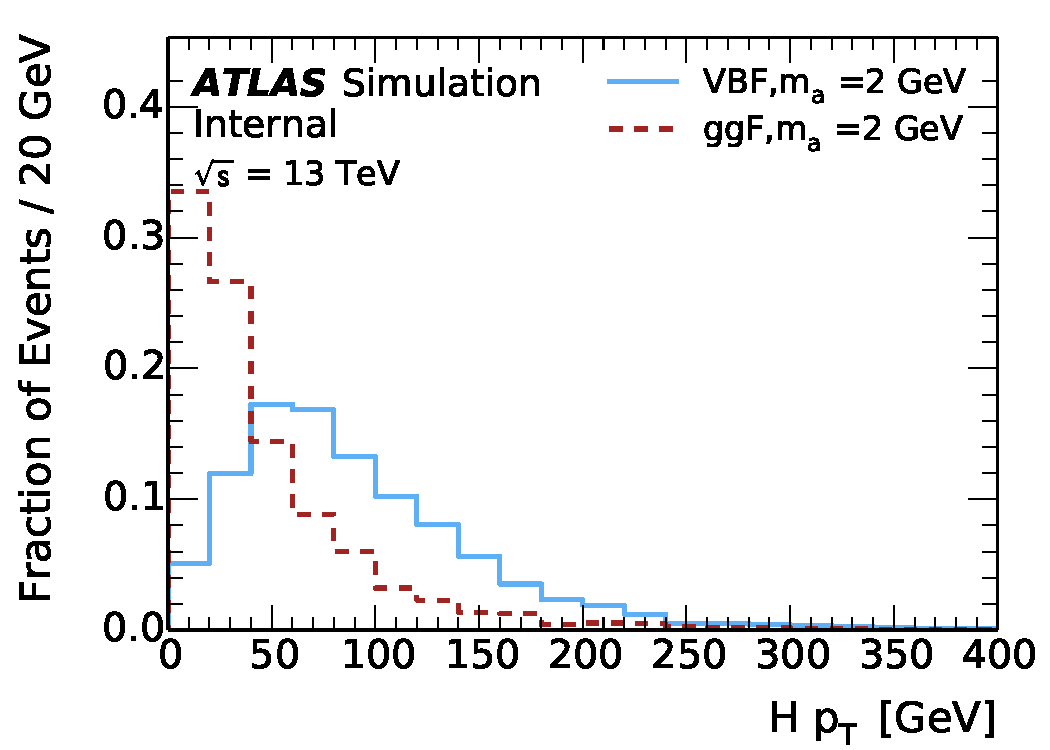
\includegraphics[width=0.25\textwidth]{{figures/H_pt_shape_a2a2.pdf}}}
  \subfloat[]{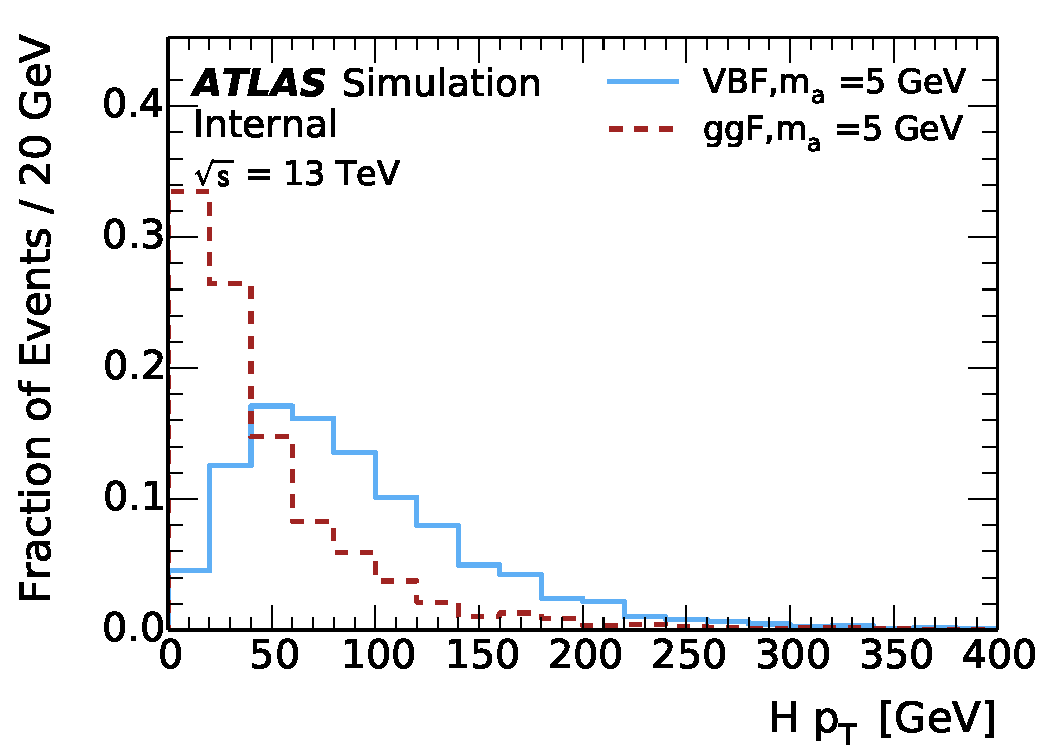
\includegraphics[width=0.25\textwidth]{{figures/H_pt_shape_a5a5.pdf}}}
  \subfloat[]{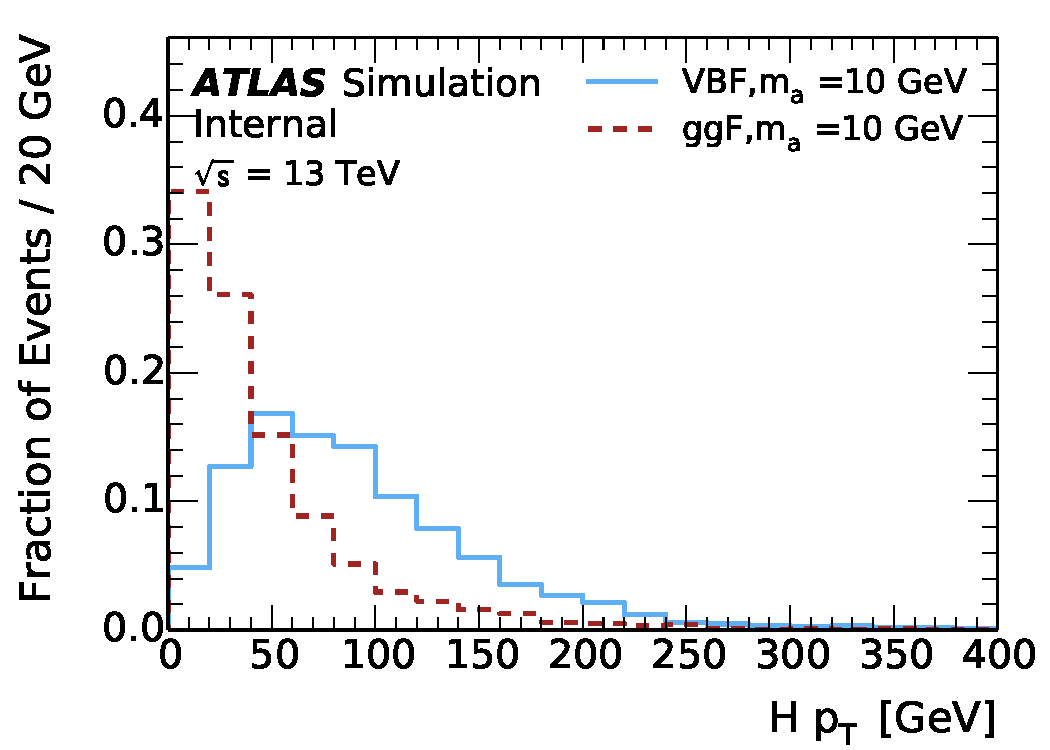
\includegraphics[width=0.25\textwidth]{{figures/H_pt_shape_a10a10.pdf}}}
  \subfloat[]{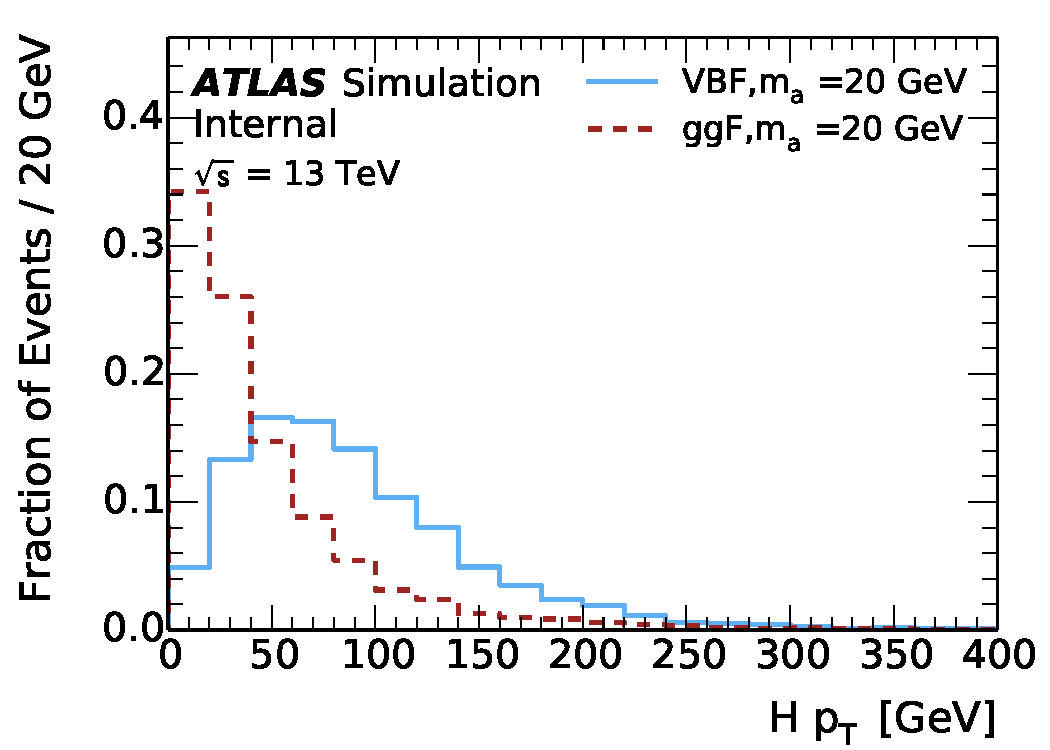
\includegraphics[width=0.25\textwidth]{{figures/H_pt_shape_a20a20.pdf}}}\\
  \subfloat[]{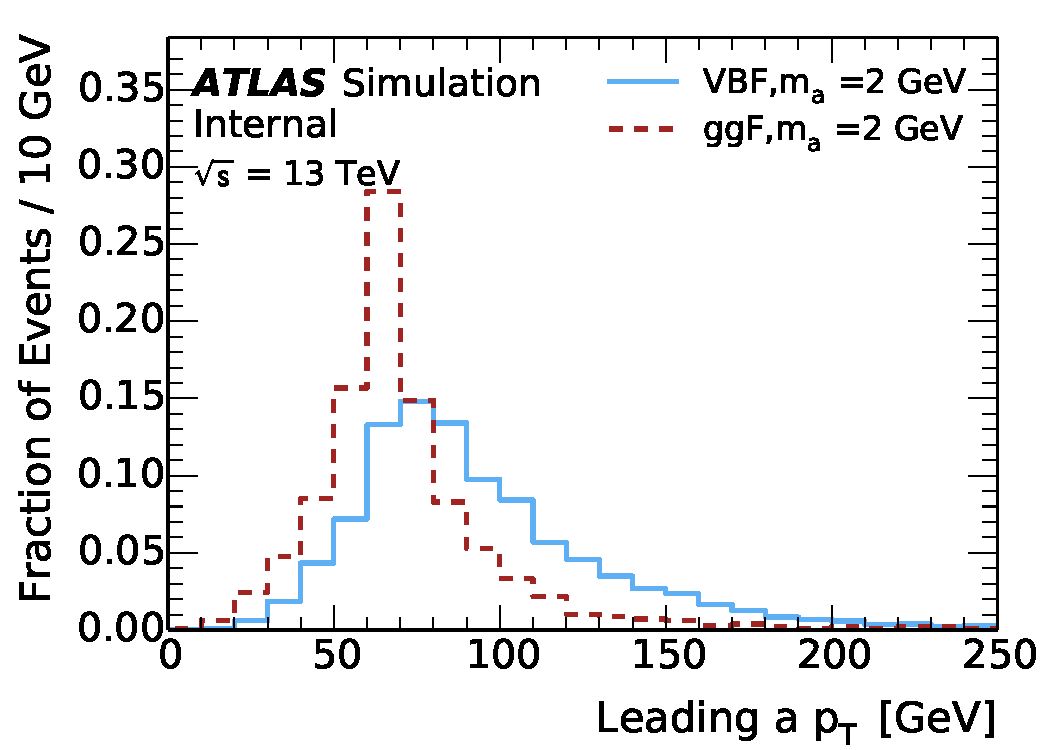
\includegraphics[width=0.25\textwidth]{{figures/a_pt1_shape_a2a2.pdf}}}
  \subfloat[]{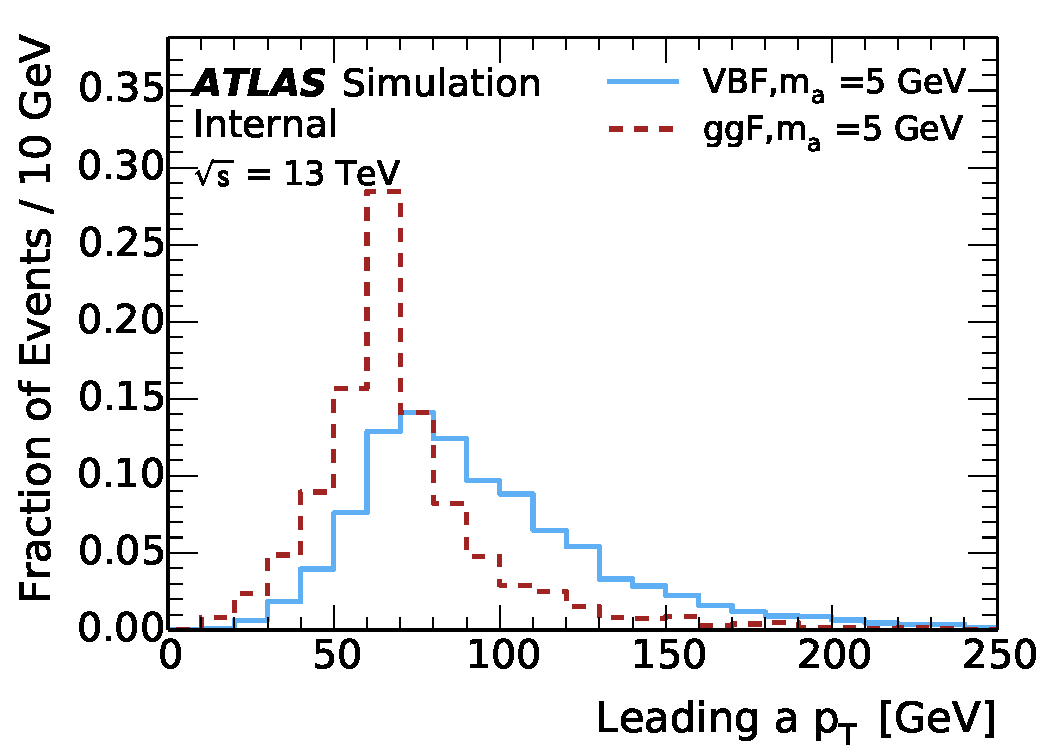
\includegraphics[width=0.25\textwidth]{{figures/a_pt1_shape_a5a5.pdf}}}
  \subfloat[]{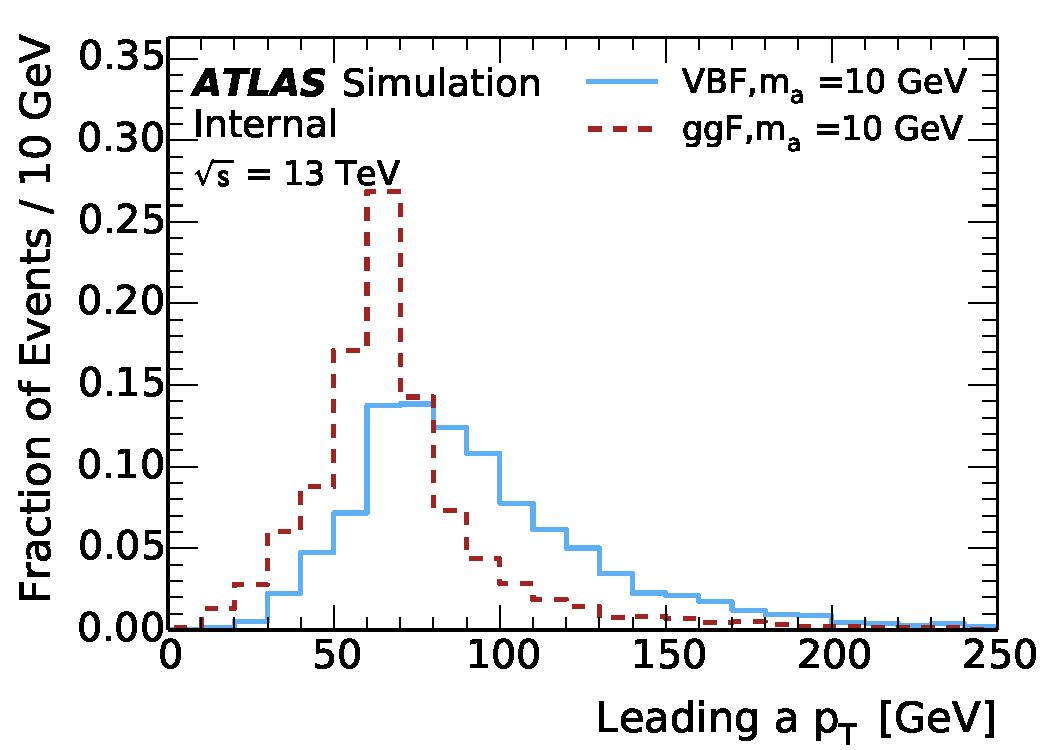
\includegraphics[width=0.25\textwidth]{{figures/a_pt1_shape_a10a10.pdf}}}
  \subfloat[]{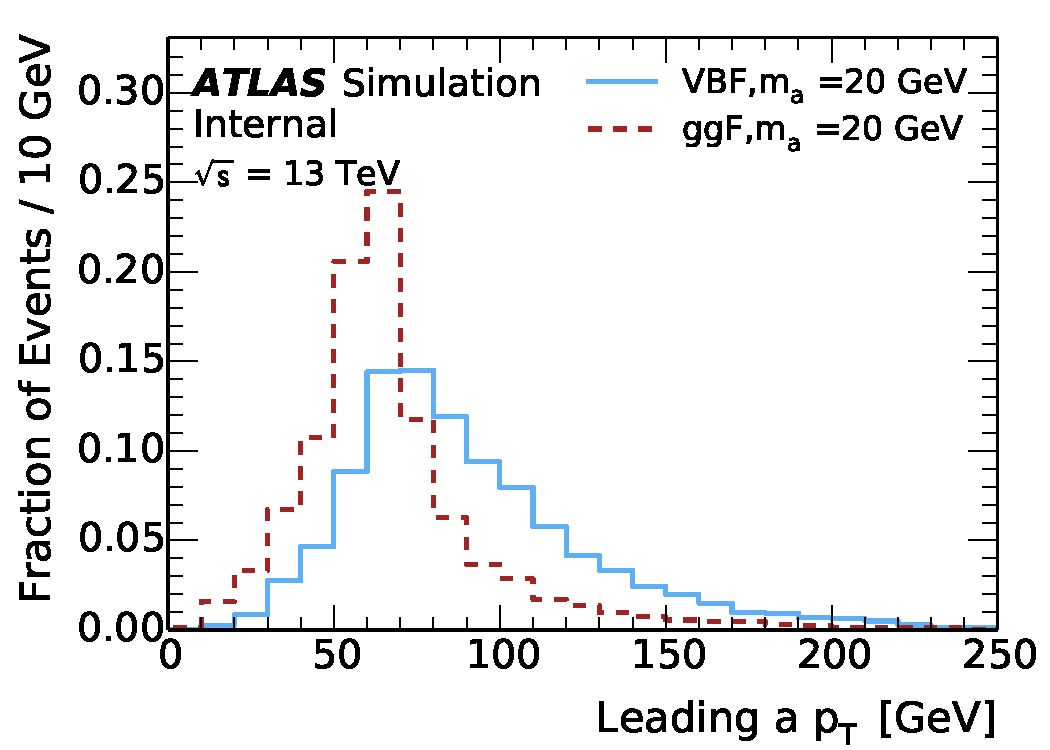
\includegraphics[width=0.25\textwidth]{{figures/a_pt1_shape_a20a20.pdf}}}\\
  \subfloat[]{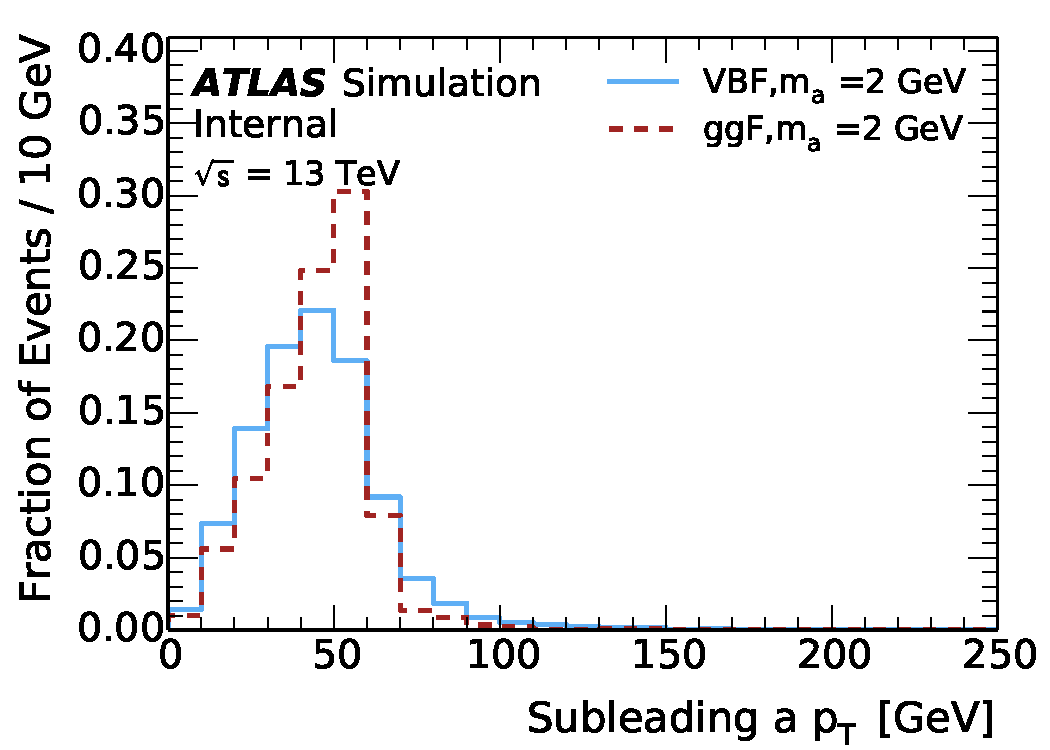
\includegraphics[width=0.25\textwidth]{{figures/a_pt2_shape_a2a2.pdf}}}
  \subfloat[]{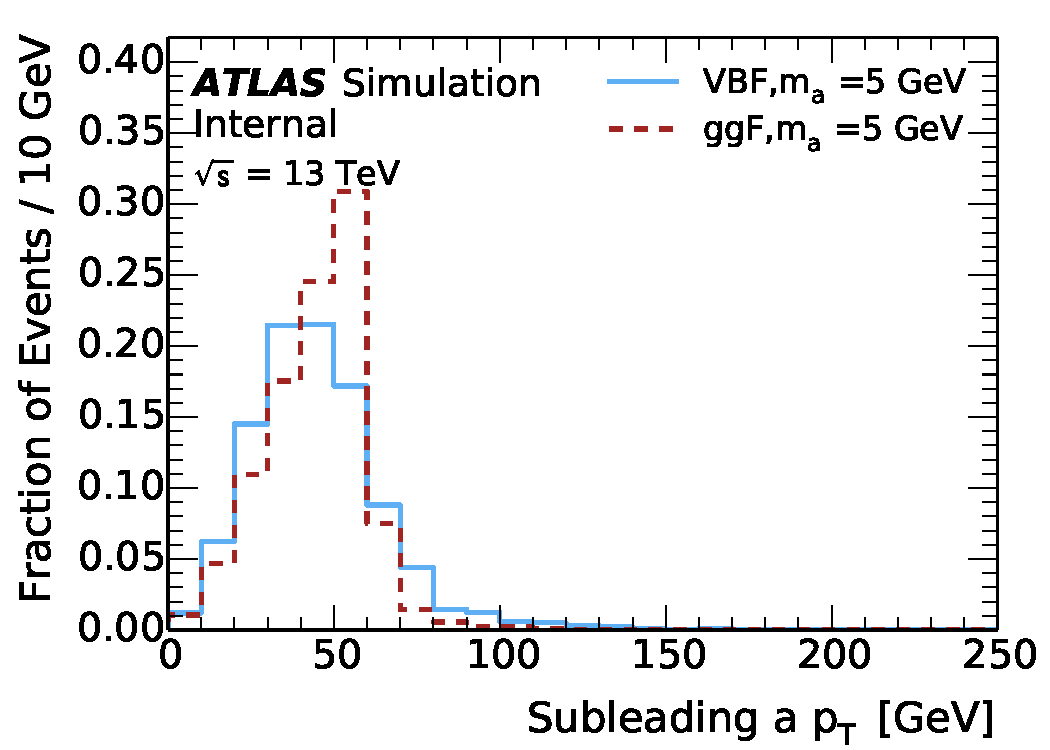
\includegraphics[width=0.25\textwidth]{{figures/a_pt2_shape_a5a5.pdf}}}
  \subfloat[]{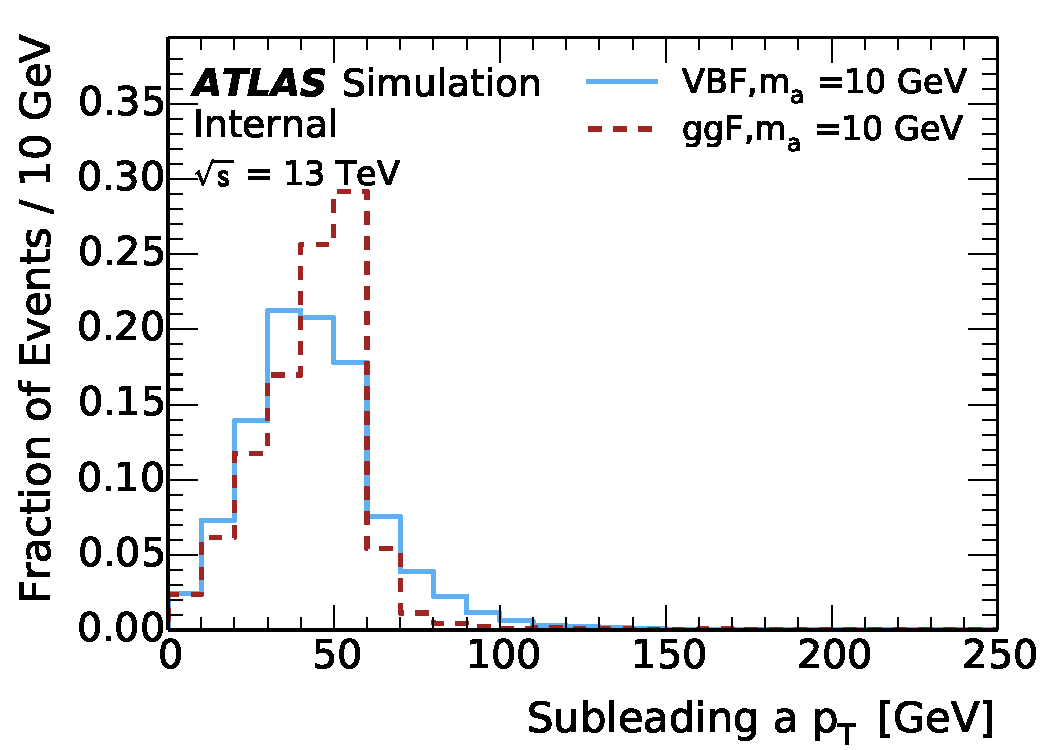
\includegraphics[width=0.25\textwidth]{{figures/a_pt2_shape_a10a10.pdf}}}
  \subfloat[]{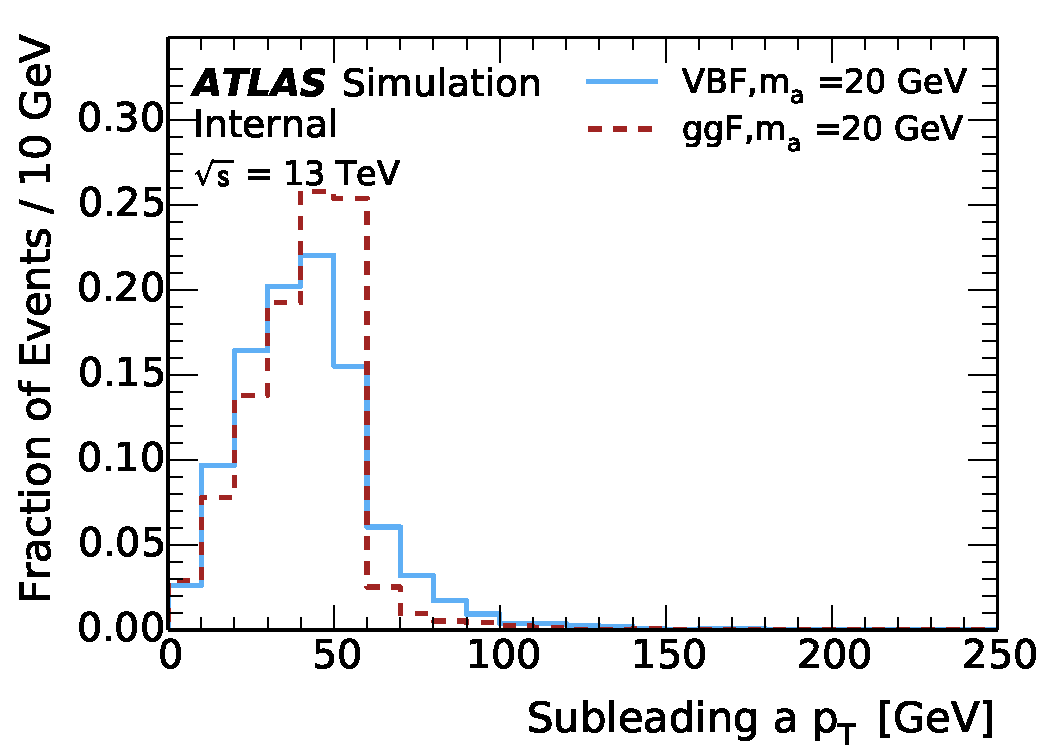
\includegraphics[width=0.25\textwidth]{{figures/a_pt2_shape_a20a20.pdf}}}\\
  \caption{
    Distributions of the \pt{} of the (top) Higgs; (middle) leading $a$; and (bottom) subleading $a$ particle, at truth level.
    The quantities are shown for simulated signal events with
    (first column) $m_a=2$ \GeV{};
    (second column) $m_a=5$ \GeV{};
    (third column) $m_a=10$ \GeV{};
    and (fourth column) $m_a=20$ \GeV{}.
    The distributions are shown separately for events produced in the VBF mode and those produced in the ggF mode.
    }
  \label{fig:HBSM_app:a_pt}
\end{figure}

This boosting can be seen in Figure~\ref{fig:HBSM_app:photons} for the photon decay products of the $a$ and in Figure~\ref{fig:HBSM_app:gluons} for the gluon decay products of the $a$.
While the \pt{} of the photons and gluon decay products are relatively unaffected by the mass of the $a$, for low $m_a$ the $\Delta R$ between the two decay products gets very small.
This dependence of $\Delta R$ on $m_a$ affects both the trigger efficiency (Section~\ref{sec:HBSM:trigger}) and the offline diphoton selection efficiency (Section~\ref{sec:HBSM:photons}).

The value $\Delta R=0.2$ is the distance metric for the photon reconstruction at the trigger level; below this value only one photon region of interest is identified~\cite{Achenbach:2008zzb,Aad:2019wsl}.
For $m_a<10$ \GeV{} it is clear that this effect ruins the trigger efficiency, since a large fraction of the events have between the two photons $\Delta R<0.2$.
For $10<m_a<20$ \GeV{} the effect is a little more nuanced.
Some fraction of the photons do have $\Delta R < 0.2$ and therefore do not pass the trigger requirement.
For the photons with $\Delta R > 0.2$, since the opening angle between the photons $\Delta R \sim \frac{2m_a}{\pt}$, the \pt{} of the originating $a$ particle is $\sim \frac{2m_a}{\Delta R} < 10 m_a$.
Assuming the \pt{} of the two decay products are chosen basically uniformly between $0$ and the \pt{} of the $a$ particle, subject to conservation of energy, the \pt{} of the leading photon is expected to be on average twice the \pt{} of the subleading photon, and therefore the \pt{} of the subleading photon is about $\frac{1}{3}$ of the \pt{} of the $a$ particle; this can be seen in Figure~\ref{fig:HBSM_app:photons} (and also in Figures~\ref{fig:HBSM_app:gluons} for the gluon decay products).
Thus, e.g. for $m_a \sim 10$ \GeV{} and $\Delta R = 0.2$, the \pt{} of the subleading photon is on average (and therefore half the time less than) $33$ \GeV{}, therefore not passing the \texttt{HLT\_g35\_loose\_g25\_loose} trigger.
Of course, for larger $\Delta R$ at fixed $m_a$ this effect gets stronger.

In summary, there are two effects that cause the photon trigger efficiency to go down for small $m_a$.
The first is simply that a larger fraction of events have the two photon decay products with $\Delta R<0.2$.
The second is that, for $\Delta R>0.2$, for fixed $m_a$ as $\Delta R$ gets larger the \pt{} of the $a$ particle and therefore of the photons goes down inversely, and around $m_a=10$ \GeV{} the subleading photon is around the trigger threshold, causing inefficiencies.
The trigger therefore requires $m_a$ to be high enough such that if the \pt{} of the $a$ particle is high enough for its decay products to pass the trigger threshold, the $\Delta R$ between the two photon decay products is also large enough to be reconstructed as two trigger-level photons.

At the offline level, $\Delta R=0.4$ is the distance metric for the photon isolation~\cite{PERF-2013-04}; below this value the photons are not reconstructed as isolated (ruining the offline selection efficiency).
However, at offline level this isolation can be turned off, and since the triggers used in this analysis have no isolation applied (though such an isolation is possible~\cite{Aad:2019wsl}), the effects of the isolation at least are not limiting the sensitivity of this analysis.
Of course, the isolation on the offline photons was kept for this search; this is due to the trigger selection limiting the efficiency on the low masses, and the higher masses tending to have $\Delta R>0.4$ so that the isolation has high signal efficiency and contributes to the background rejection.

Finally, the value $\Delta R=0.4$ is the distance metric for the small-R jet algorithm; below this value both the photons and gluons are reconstructed in a single jet (making the offline selection significantly harder).
\begin{figure}[t]
  \centering 
  \subfloat[]{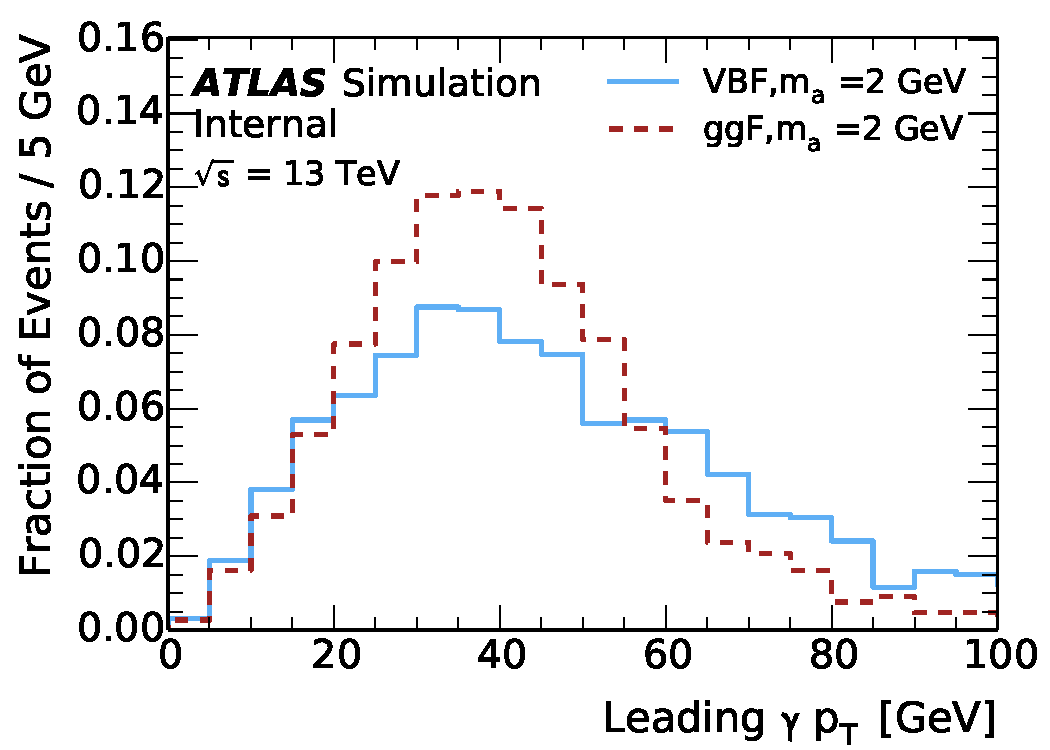
\includegraphics[width=0.25\textwidth]{{figures/y_pt1_shape_a2a2.pdf}}}
  \subfloat[]{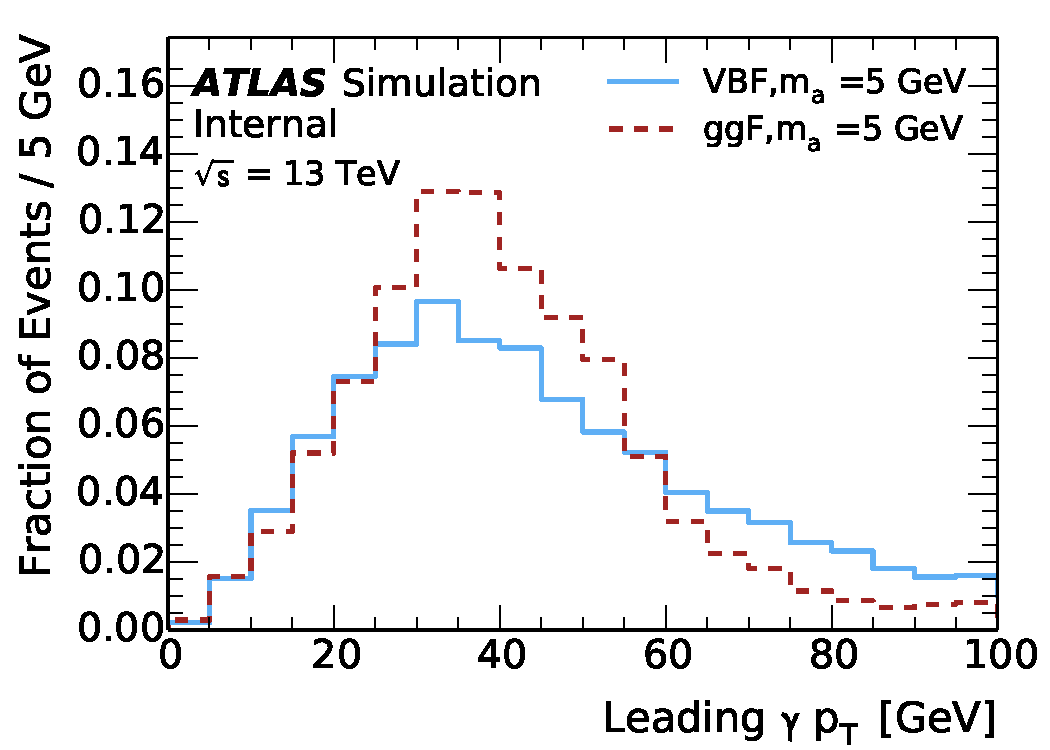
\includegraphics[width=0.25\textwidth]{{figures/y_pt1_shape_a5a5.pdf}}}
  \subfloat[]{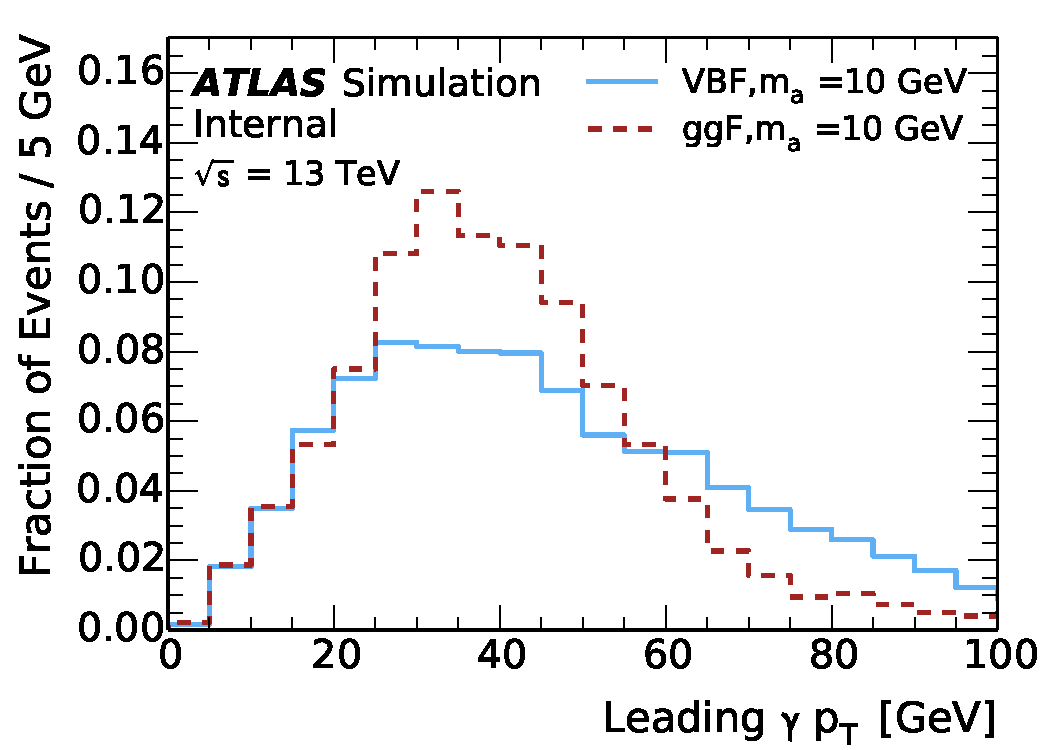
\includegraphics[width=0.25\textwidth]{{figures/y_pt1_shape_a10a10.pdf}}}
  \subfloat[]{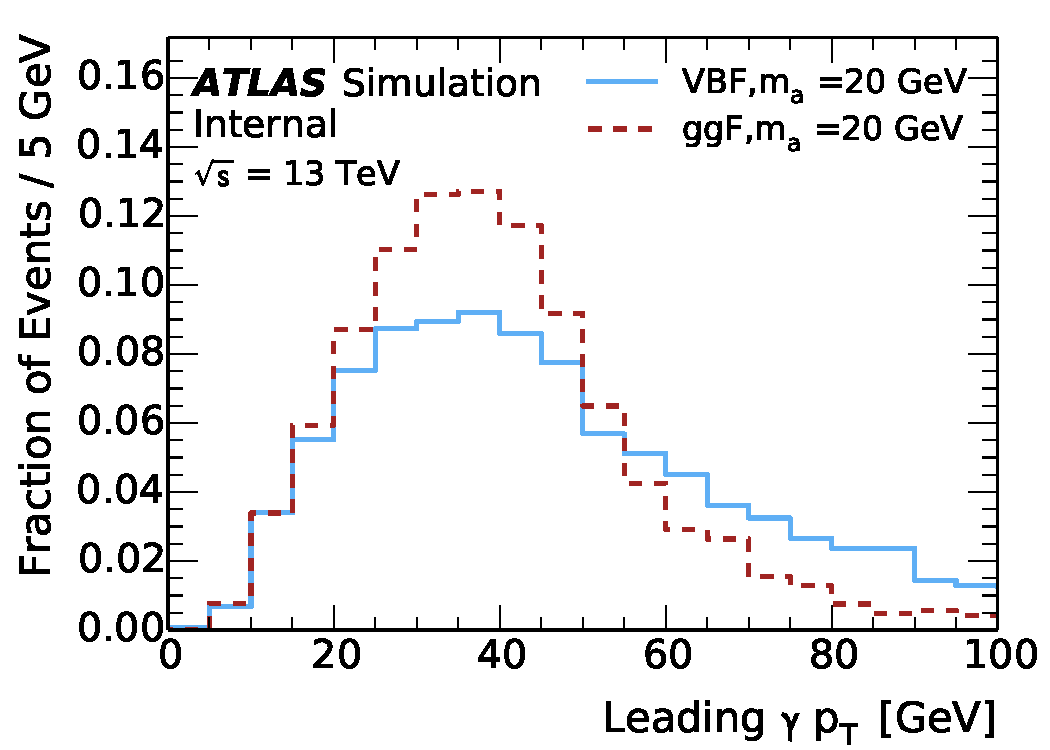
\includegraphics[width=0.25\textwidth]{{figures/y_pt1_shape_a20a20.pdf}}}\\
  \subfloat[]{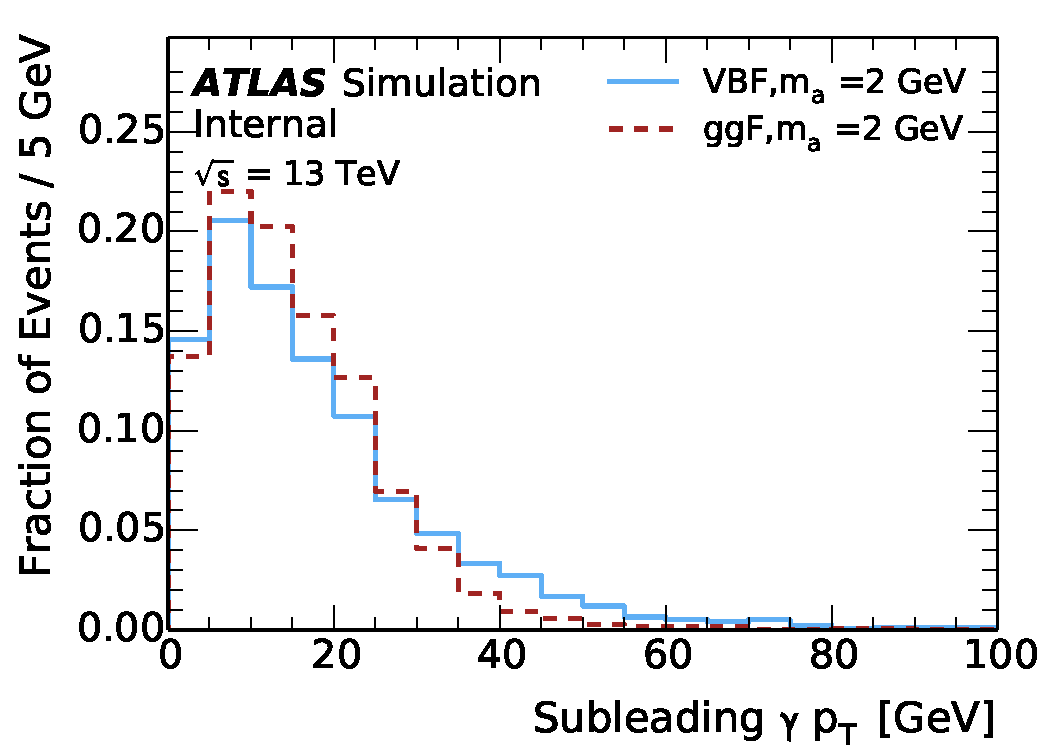
\includegraphics[width=0.25\textwidth]{{figures/y_pt2_shape_a2a2.pdf}}}
  \subfloat[]{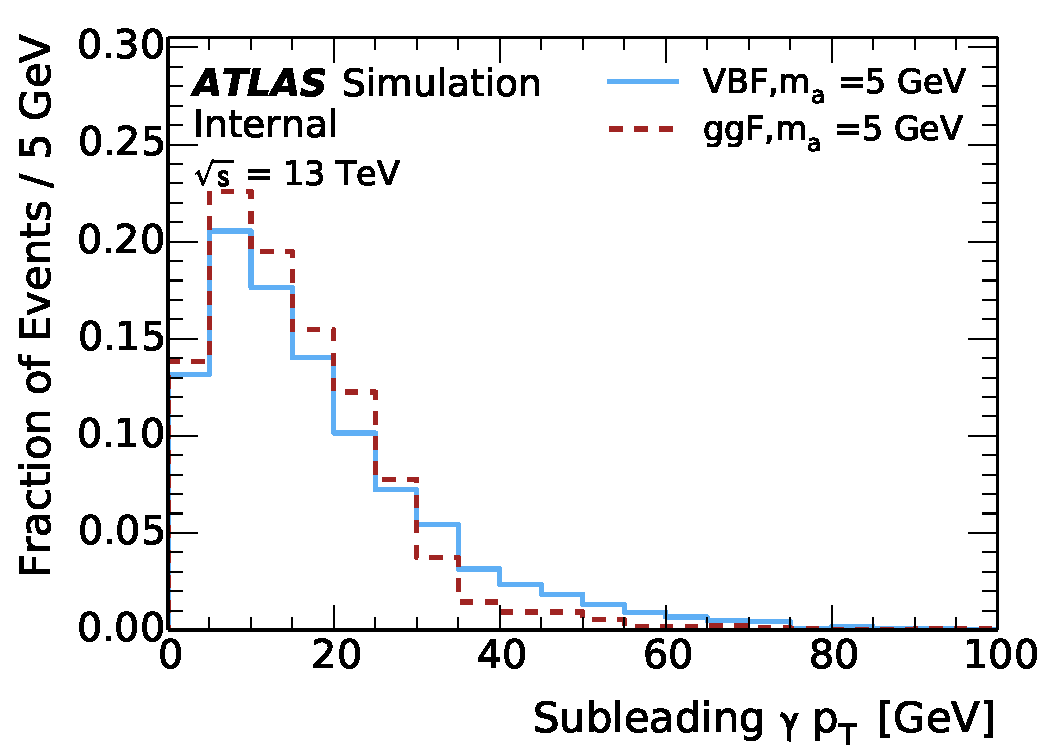
\includegraphics[width=0.25\textwidth]{{figures/y_pt2_shape_a5a5.pdf}}}
  \subfloat[]{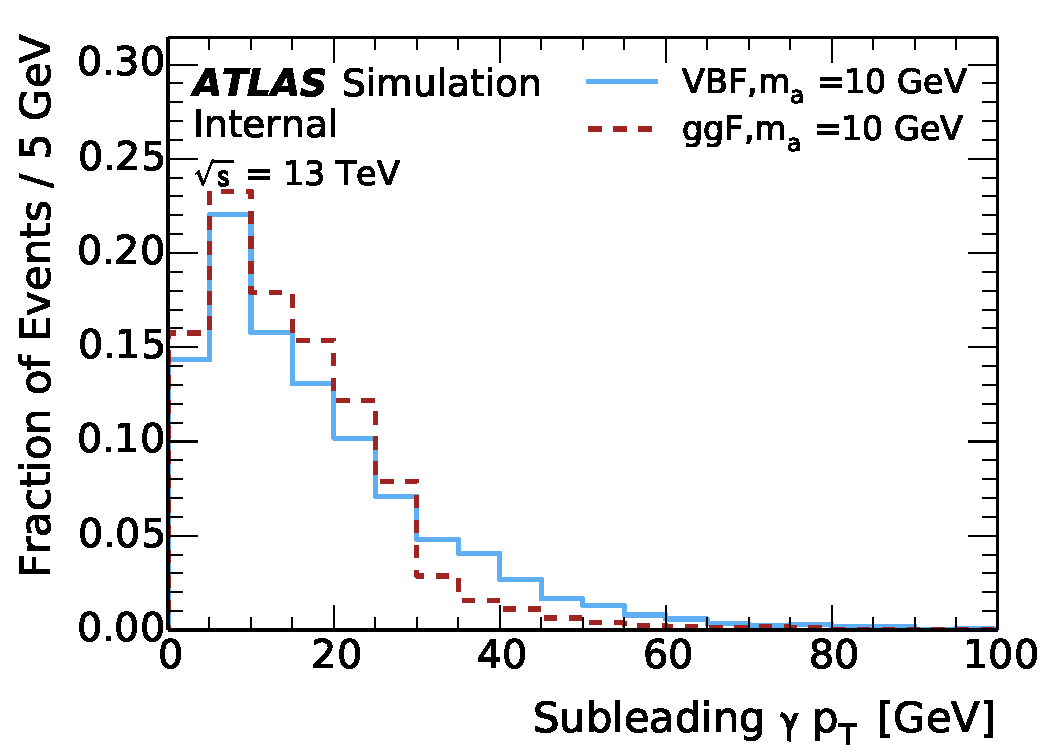
\includegraphics[width=0.25\textwidth]{{figures/y_pt2_shape_a10a10.pdf}}}
  \subfloat[]{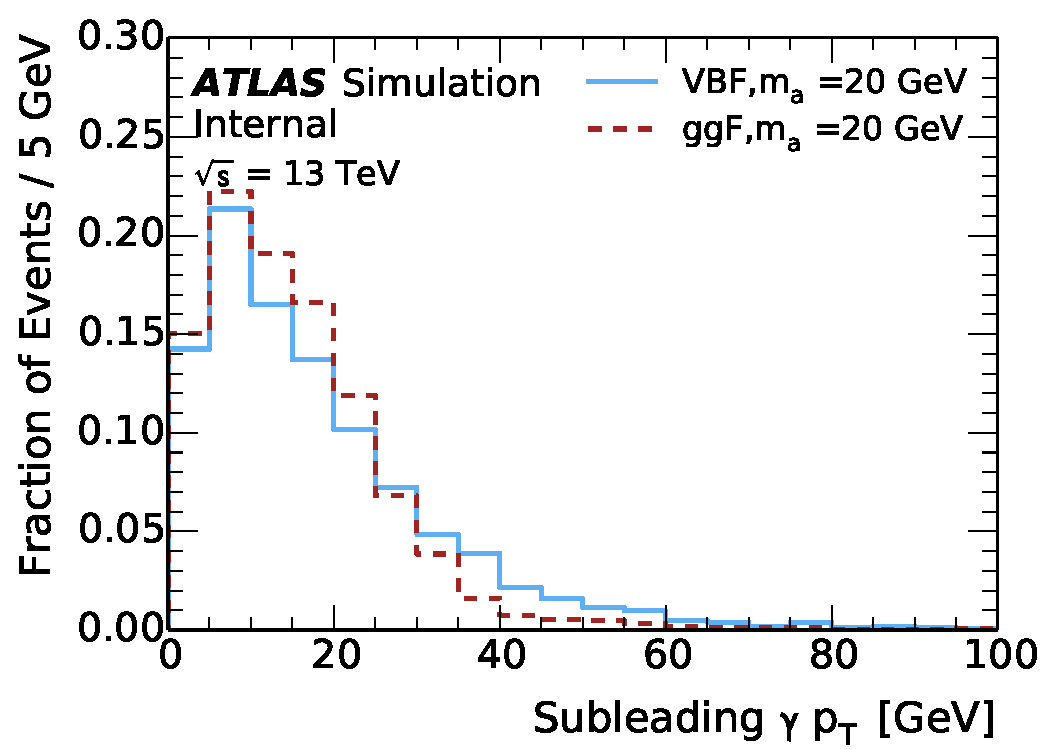
\includegraphics[width=0.25\textwidth]{{figures/y_pt2_shape_a20a20.pdf}}}\\
  \subfloat[]{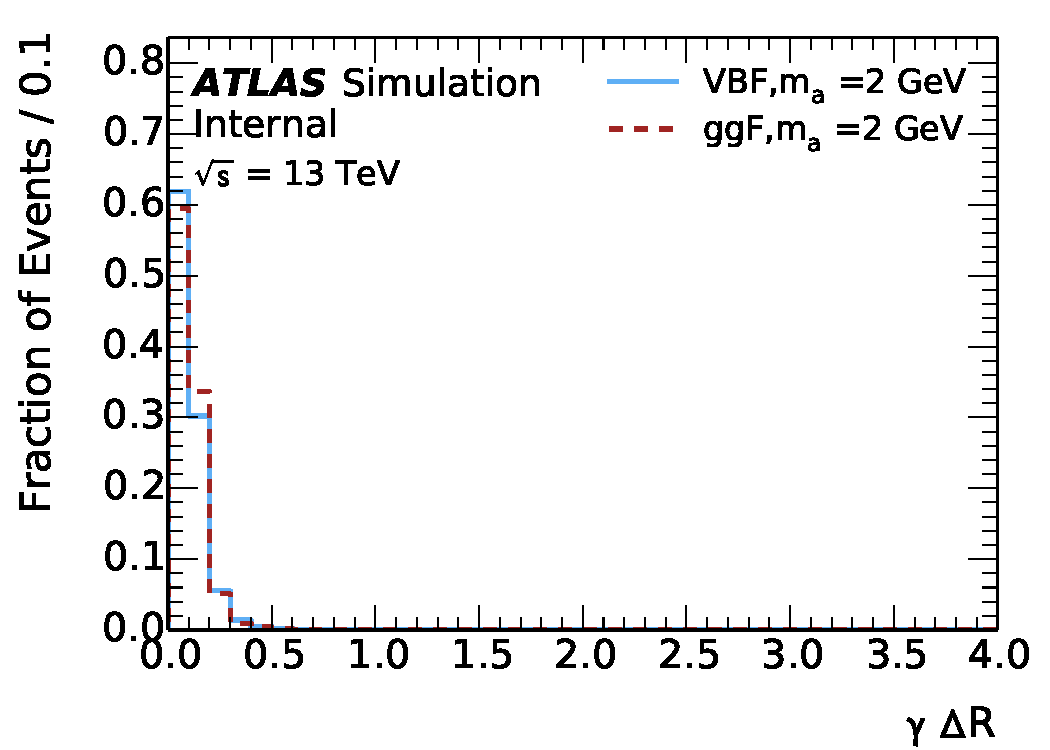
\includegraphics[width=0.25\textwidth]{{figures/y_dR_shape_a2a2.pdf}}}
  \subfloat[]{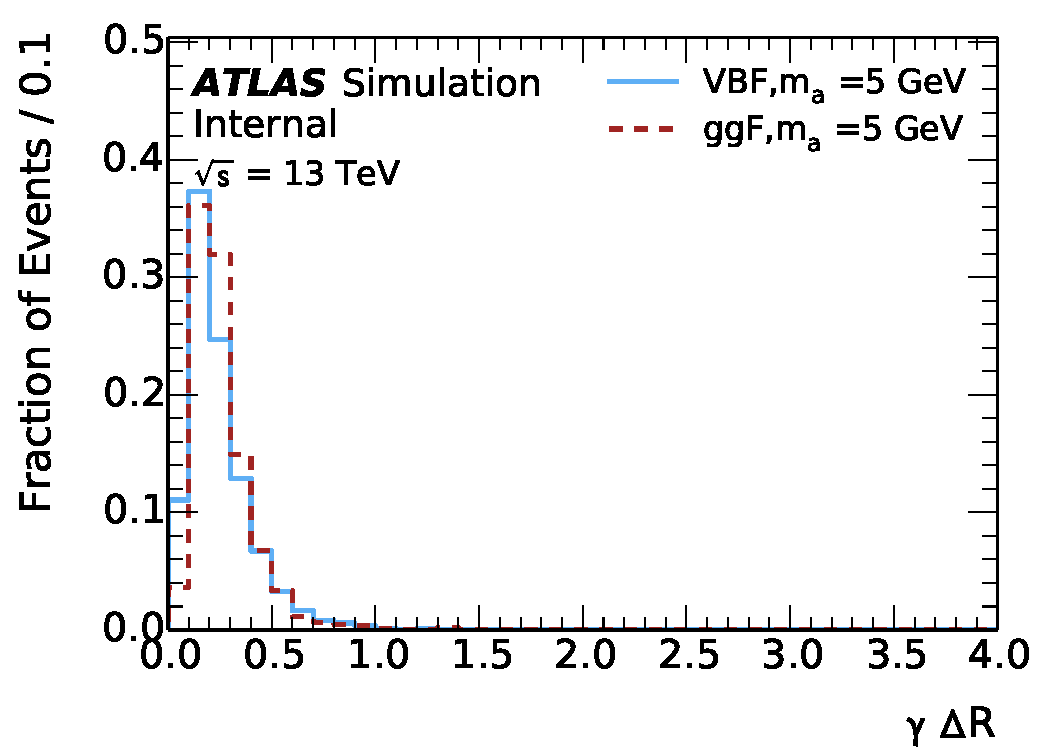
\includegraphics[width=0.25\textwidth]{{figures/y_dR_shape_a5a5.pdf}}}
  \subfloat[]{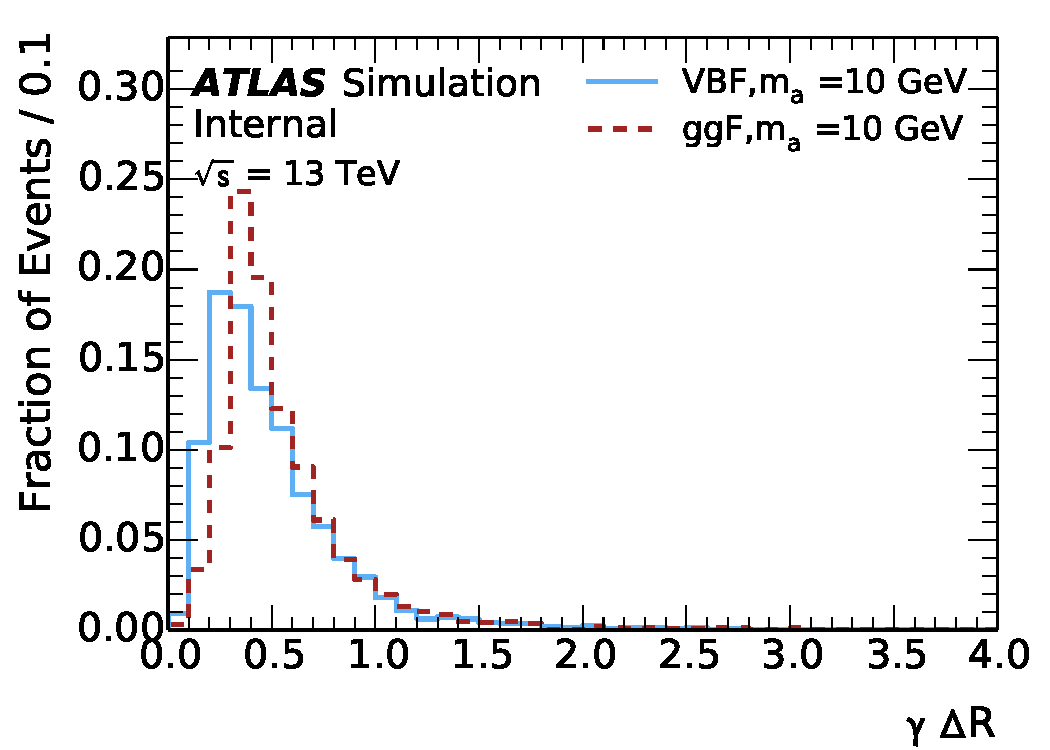
\includegraphics[width=0.25\textwidth]{{figures/y_dR_shape_a10a10.pdf}}}
  \subfloat[]{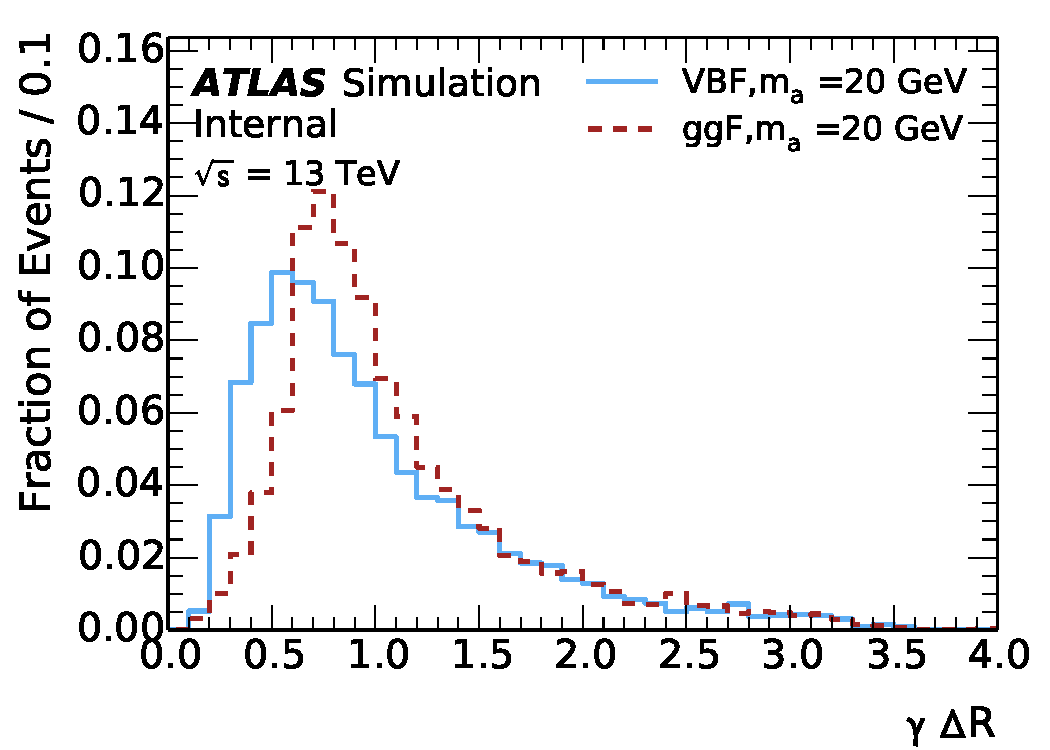
\includegraphics[width=0.25\textwidth]{{figures/y_dR_shape_a20a20.pdf}}}\\
  \caption{
    Distributions of the \pt{} of the (top) leading photon; (middle) subleading photon; and (bottom) $\Delta R$ between the two photons, at truth level.
    The quantities are shown for simulated signal events with
    (first column) $m_a=2$ \GeV{};
    (second column) $m_a=5$ \GeV{};
    (third column) $m_a=10$ \GeV{};
    and (fourth column) $m_a=20$ \GeV{}.
    The distributions are shown separately for events produced in the VBF mode and those produced in the ggF mode.
    }
  \label{fig:HBSM_app:photons}
\end{figure}
\begin{figure}[t]
  \centering 
  \subfloat[]{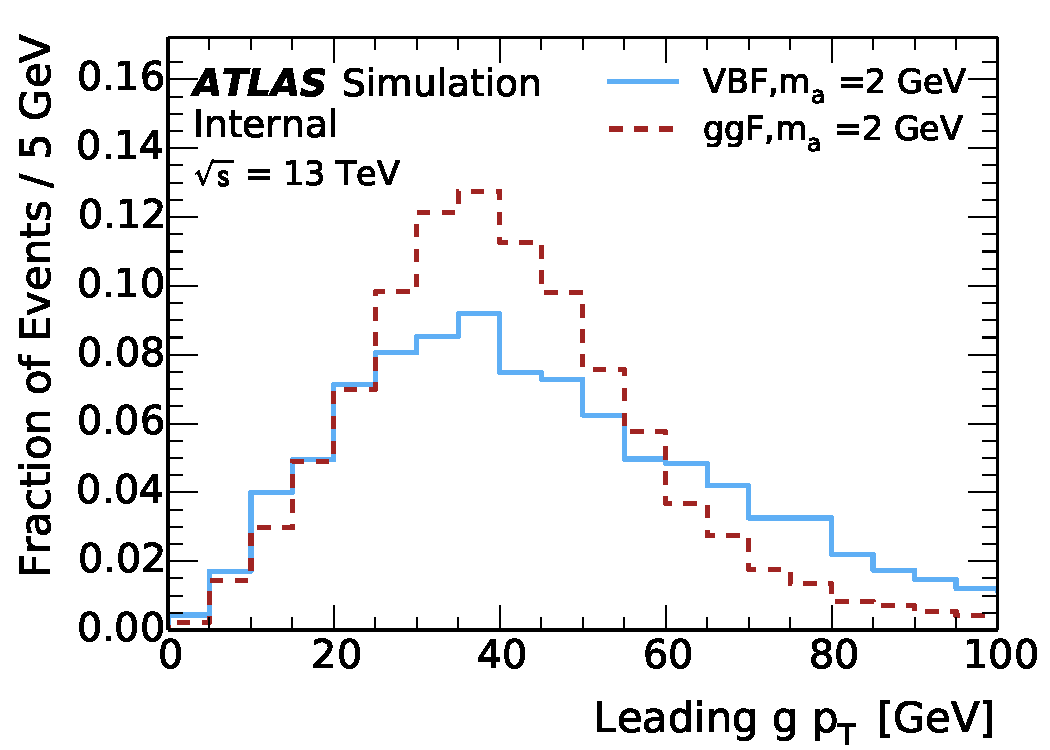
\includegraphics[width=0.25\textwidth]{{figures/g_pt1_shape_a2a2.pdf}}}
  \subfloat[]{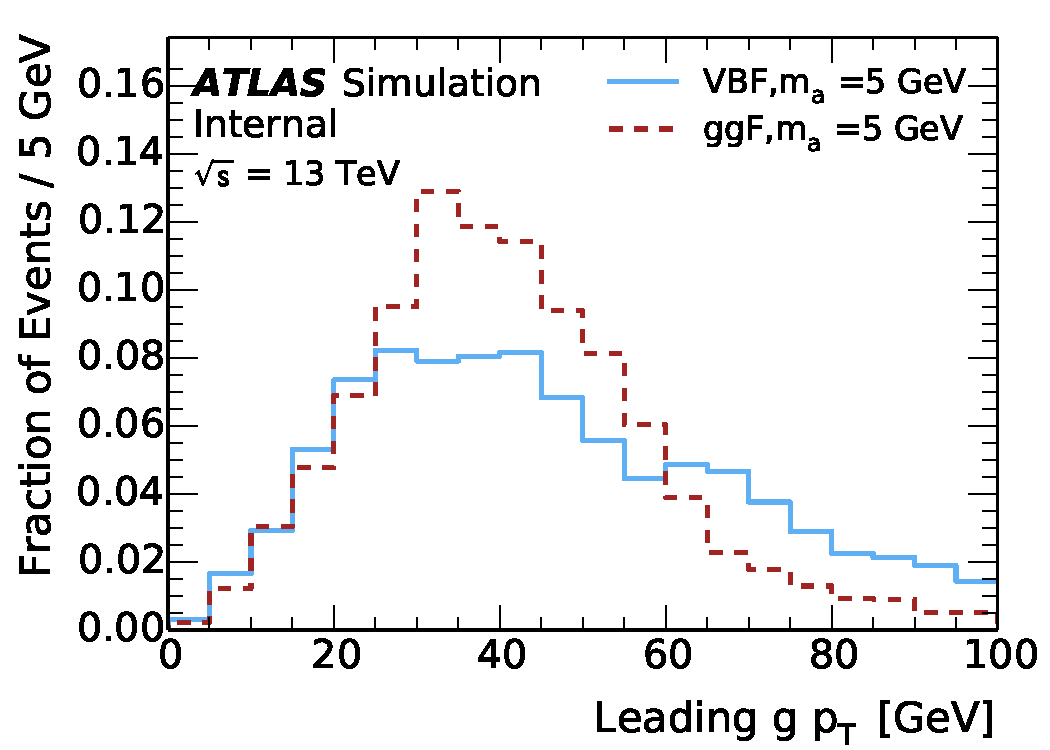
\includegraphics[width=0.25\textwidth]{{figures/g_pt1_shape_a5a5.pdf}}}
  \subfloat[]{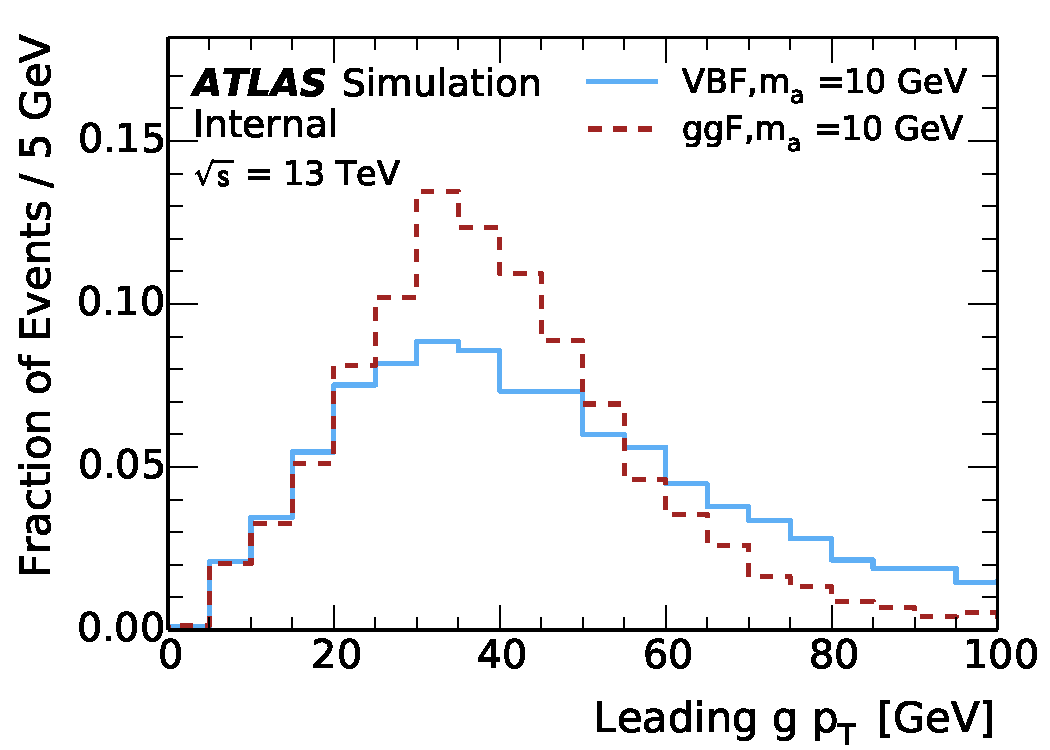
\includegraphics[width=0.25\textwidth]{{figures/g_pt1_shape_a10a10.pdf}}}
  \subfloat[]{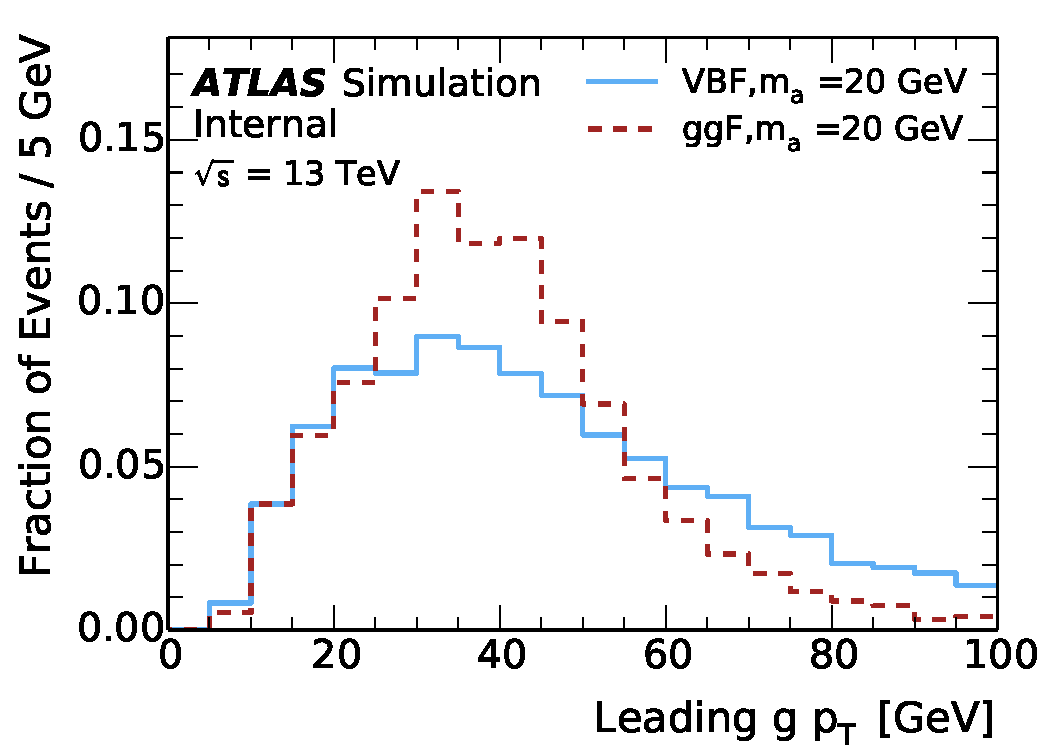
\includegraphics[width=0.25\textwidth]{{figures/g_pt1_shape_a20a20.pdf}}}\\
  \subfloat[]{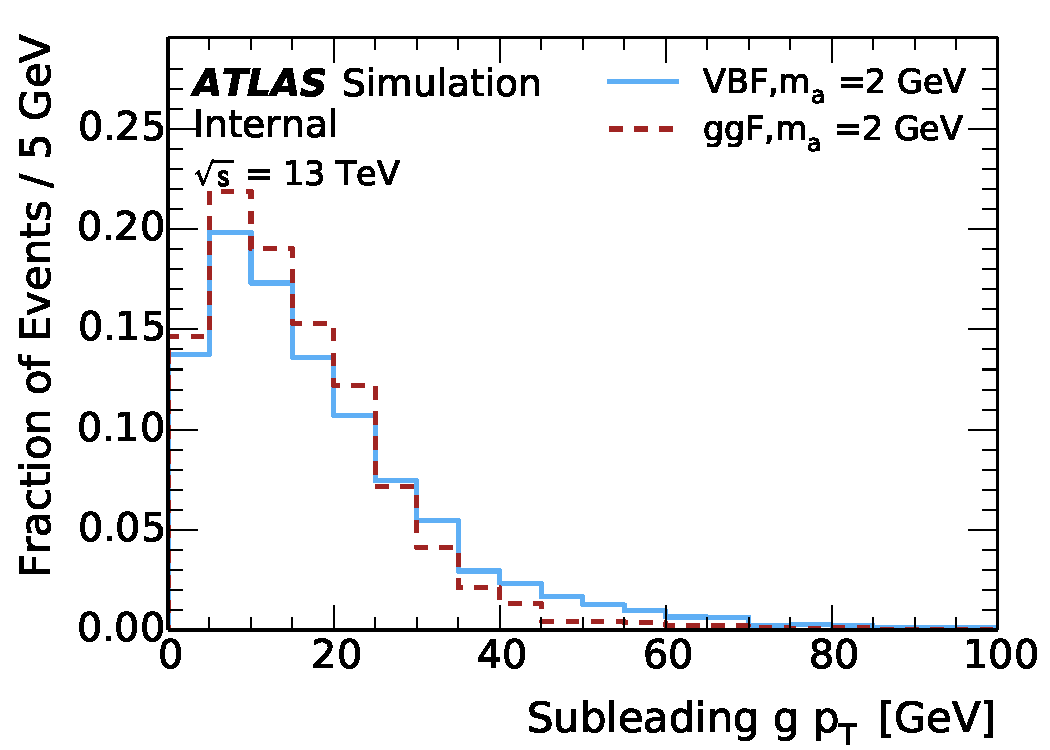
\includegraphics[width=0.25\textwidth]{{figures/g_pt2_shape_a2a2.pdf}}}
  \subfloat[]{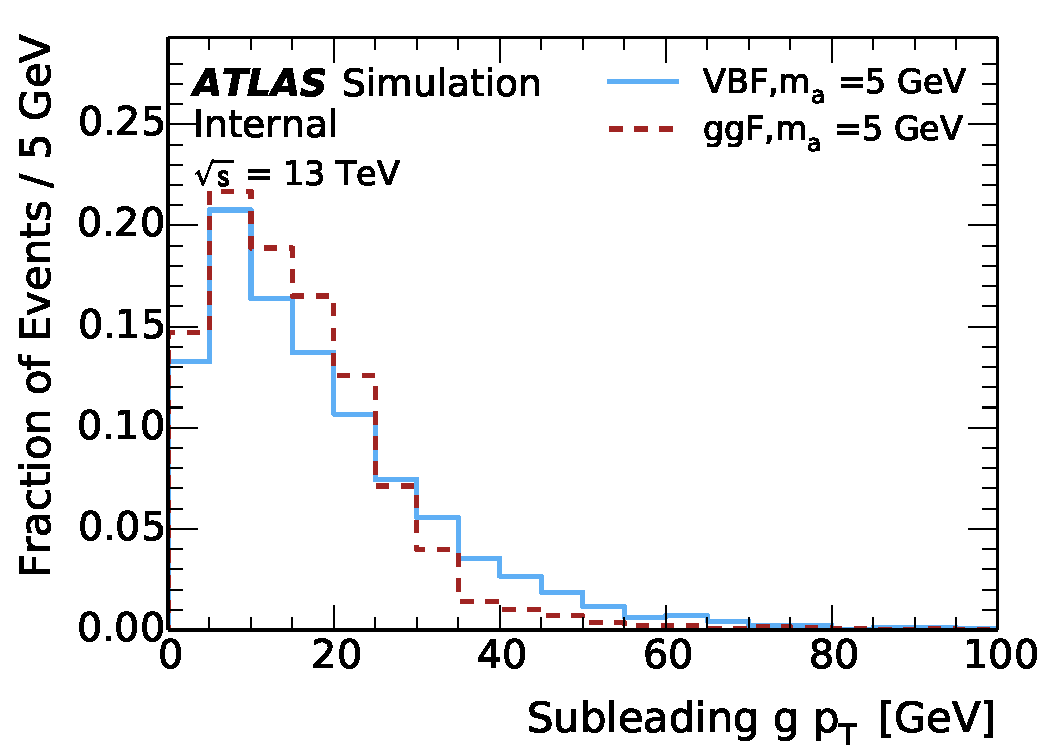
\includegraphics[width=0.25\textwidth]{{figures/g_pt2_shape_a5a5.pdf}}}
  \subfloat[]{\includegraphics[width=0.25\textwidth]{{figures/g_pt2_shape_a10a10.pdf}}}
  \subfloat[]{\includegraphics[width=0.25\textwidth]{{figures/g_pt2_shape_a20a20.pdf}}}\\
  \subfloat[]{\includegraphics[width=0.25\textwidth]{{figures/g_dR_shape_a2a2.pdf}}}
  \subfloat[]{\includegraphics[width=0.25\textwidth]{{figures/g_dR_shape_a5a5.pdf}}}
  \subfloat[]{\includegraphics[width=0.25\textwidth]{{figures/g_dR_shape_a10a10.pdf}}}
  \subfloat[]{\includegraphics[width=0.25\textwidth]{{figures/g_dR_shape_a20a20.pdf}}}\\
  \caption{
    Distributions of the \pt{} of the (top) leading signal gluon; (middle) subleading signal gluon; and (bottom) $\Delta R$ between the two gluons, at truth level.
    The quantities are shown for simulated signal events with
    (first column) $m_a=2$ \GeV{};
    (second column) $m_a=5$ \GeV{};
    (third column) $m_a=10$ \GeV{};
    and (fourth column) $m_a=20$ \GeV{}.
    The distributions are shown separately for events produced in the VBF mode and those produced in the ggF mode.
    }
  \label{fig:HBSM_app:gluons}
\end{figure}

However, there is an existing trigger which can be sensitive to these boosted topologies.
This trigger is seeded off the L1 trigger that requires a single isolated photon with $\et{} > 22$ \GeV{}.
In the high-level trigger, there are three additional requirements: a photon with $\et{} > 25$ GeV; at least four jets with $\et{} > 35$ GeV and $|\eta| <4.9$; and at least one dijet pair with invariant mass greater than $1000$ \GeV{}.
In ATLAS nomenclature, this trigger is called \texttt{HLT\_g25\_medium\_4j35\_0eta490\_invm1000\_L1\_EM22VHI}.
That this trigger has efficiency on our signals is an accident; it was originally intended for background studies for the VBF $H\rightarrow bb$ + photon analysis~\cite{Aaboud:2018gay}.
However, because of this other analysis need, this trigger was running in 2015-2018 data-taking periods~\cite{unprescaledwiki,ATL-DAQ-PUB-2016-001,ATL-DAQ-PUB-2017-001,ATL-DAQ-PUB-2018-002,ATL-DAQ-PUB-2019-001}.

This trigger has potential to be efficient on our signals at low $m_a$.
First, the photon isolation at L1 only goes out to $\Delta R=0.2$~\cite{Aad:2019wsl}; and furthermore, no isolation at all is applied if the \pt{} of the photon is $>50$ \GeV{}.
As argued above, for fixed $m_a$ as $\Delta R$ between the photons gets smaller the \pt{} of the leading photon gets larger, so that these two effects can mostly cancel out and allow our signals to pass the L1 trigger.
The top row of Figure~\ref{fig:HBSM_app:turnons} shows the efficiency of this trigger as a function of the leading offine photon \pt{}; the efficiency goes to 100\% for $\pt{}>30$ \GeV{} for $m_a \ge 10$ \GeV{}, indicating that the leading photon is passing the trigger requirement.
For $m_a=2$ \GeV{}, the efficiency only goes to 100\% for $\pt{}>50$ \GeV{}, in accord with the isolation requirements mentioned above.

Second, for the VBF signals the decay products of each of the two $a$ particles are reconstructed as a single jet in the HLT (photons are reconstructed as jets both at trigger level and offline); these two jets plus the two VBF jets reach the requirement of 4 jets with $\pt{}>35$ \GeV{}, and in particular the \pt{} of each of the signal jets contains the full \pt{} of each of the $a$ particles rather than just one of the decay products.
The middle row of Figure~\ref{fig:HBSM_app:turnons} shows the efficiency of this trigger as a function of the 4th-leading offine jet \pt{} (including jets overlapping photons); the efficiency goes to 100\% for $\pt{}>40$ \GeV{}, indicating that the photons are being picked up as jets in the HLT.

Finally, the photon in the HLT requirement is met by the leading photon, since no isolation is required at HLT; and the invariant mass requirement is of course met in the VBF topology.
The bottom row of Figure~\ref{fig:HBSM_app:turnons} shows the efficiency of this trigger as a function of the maximum dijet invariant mass; the efficiency goes to 100\% for invariant mass $>1100$ \GeV{}, indicating the level at which the turnon occurs.

\begin{figure}[t]
  \centering 
  \subfloat[]{\includegraphics[width=0.25\textwidth]{{figures/turnon_HLT_g25_medium_L1EM22VHI_4j35_0eta490_invm1000_gpt_ma2.pdf}}}
  \subfloat[]{\includegraphics[width=0.25\textwidth]{{figures/turnon_HLT_g25_medium_L1EM22VHI_4j35_0eta490_invm1000_gpt_ma10.pdf}}}
  \subfloat[]{\includegraphics[width=0.25\textwidth]{{figures/turnon_HLT_g25_medium_L1EM22VHI_4j35_0eta490_invm1000_gpt_ma20.pdf}}}\\
  \subfloat[]{\includegraphics[width=0.25\textwidth]{{figures/turnon_HLT_g25_medium_L1EM22VHI_4j35_0eta490_invm1000_j4_ma2.pdf}}}
  \subfloat[]{\includegraphics[width=0.25\textwidth]{{figures/turnon_HLT_g25_medium_L1EM22VHI_4j35_0eta490_invm1000_j4_ma10.pdf}}}
  \subfloat[]{\includegraphics[width=0.25\textwidth]{{figures/turnon_HLT_g25_medium_L1EM22VHI_4j35_0eta490_invm1000_j4_ma20.pdf}}}\\
  \subfloat[]{\includegraphics[width=0.25\textwidth]{{figures/turnon_HLT_g25_medium_L1EM22VHI_4j35_0eta490_invm1000_mjj_ma2.pdf}}}
  \subfloat[]{\includegraphics[width=0.25\textwidth]{{figures/turnon_HLT_g25_medium_L1EM22VHI_4j35_0eta490_invm1000_mjj_ma10.pdf}}}
  \subfloat[]{\includegraphics[width=0.25\textwidth]{{figures/turnon_HLT_g25_medium_L1EM22VHI_4j35_0eta490_invm1000_mjj_ma20.pdf}}}
  \caption{
    Efficiency of the \texttt{HLT\_g25\_medium\_4j35\_0eta490\_invm1000} trigger on VBF signal events with (left) $m_a=2$ \GeV{}; (middle) $m_a=10$ \GeV{}; and (right) $m_a=20$ \GeV{}.
    The efficiency is shown as a function of (top) the leading offline photon \pt{}; (middle) the 4th-leading offline jet including those overlapping photons; and (bottom) maximum invariant mass between any pair of offline jets.
    For each efficiency plot, all the other offline requirements shown in Table~\ref{tab:HBSM_app:new_preselection} are included, so that the efficiency reaches 100\% for large values.
    }
  \label{fig:HBSM_app:turnons}
\end{figure}

In summary, with an offline selection of at least one photon with $\pt{}>30$ \GeV{}, at least 4 jets (including any that overlap photons) with $\pt{}>40$ \GeV{}, and a maximum invariant mass of $>1100$ \GeV{}, the \texttt{HLT\_g25\_medium\_4j35\_0eta490\_invm1000} trigger is fully efficienct.
This offline selection is listed in Table~\ref{tab:HBSM_app:new_preselection}.
\begin{table}[htbp]
  \begin{center}
  \caption{Preselection for low $m_a$ analysis.}
  \label{tab:HBSM_app:new_preselection}
    {\footnotesize
  \begin{tabular}{ l c }
    \toprule
    & Selection \\
    \midrule
    Trigger & \texttt{HLT\_g25\_medium\_4j35\_0eta490\_invm1000} \\
    \\
    Photon Selection  & $\geq1$ photon with $\pt{}>30$ \GeV{} \\
    \\ 
    Jet Selection  & $\geq4$ jets (not overlap-removed) with $\pt{}>40$ \GeV{} \\
    \\ 
    Invariant Mass  & $\geq1$ pair of jets with invariant mass $>1100$ \GeV{} \\
    \\ 
    \bottomrule
  \end{tabular}
    }
  \end{center}
\end{table}

The efficiency of this offline selection on some given values of $m_a$ are shown in Table~\ref{tab:HBSM_app:new_preselection_eff}.
\begin{table}[htbp]
  \begin{center}
  \caption{Efficiency of preselection for low $m_a$ analysis.}
  \label{tab:HBSM_app:new_preselection_eff}
    {\footnotesize
  \begin{tabular}{ l c }
    \toprule
    $m_a$ [\GeV{}] & Efficiency \\
    \midrule
    2 & 0.022 \\
    10 & 0.045 \\
    20 & 0.041 \\
    \bottomrule
  \end{tabular}
    }
  \end{center}
\end{table}
These efficiencies are pretty good, considering the very tight invariant mass cut.
For comparison, for the high $m_a$ analysis, the efficiency through the trigger and VBF selection is roughly $0.02$ (Figure~\ref{fig:HBSM:cutflow_ma}).
